\section{Logic}

\subsection{Block definition diagram}
Blokdiagrammer giver et indblik på den overordnede strukturen af \textit{Konditioneringsapparatet}.  Hver kasse skal ses som en del der indgår i systemet

\subsection{Domænemodel}
Diagrammer beskriver det systemet som helhed. Ved gennemgang af alle use cases findes væsentlig navneord og disse oprettet som konceptuelle klasser. Det konceptuelle klasser er derefter oversat til engelsk

\subsection{State machine diagram}

\subsubsection{Boot}
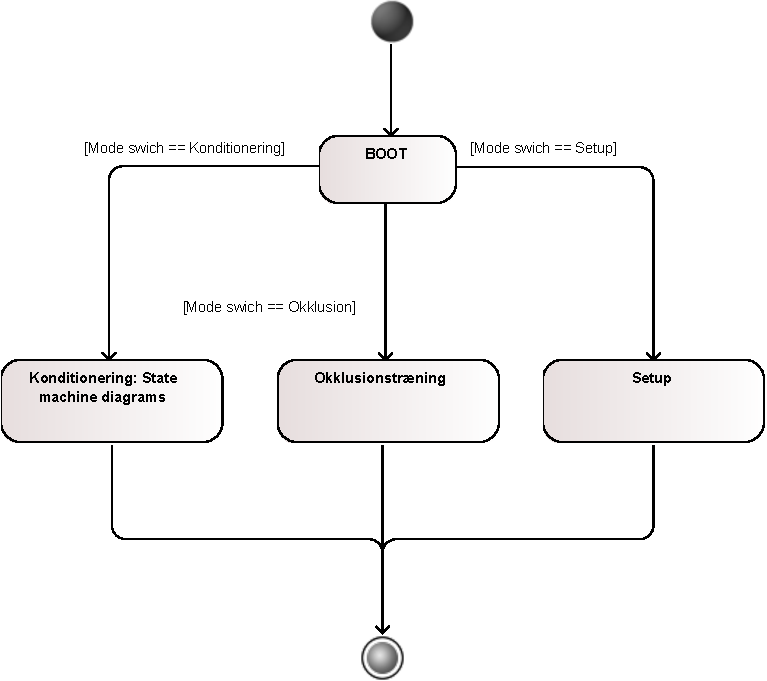
\includegraphics[width=\textwidth]{pdfs/STM_BOOT-crop.pdf} 

\subsubsection{Konditionering}
Ved knap tryk på [Start/Stop] \\
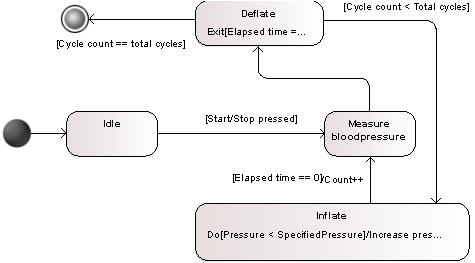
\includegraphics[width=\textwidth]{pdfs/STM_Konditionering1-crop.pdf}

Ved knap tryk på [Mål blodtryk] \\
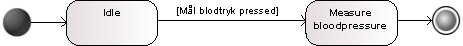
\includegraphics[width=\textwidth]{pdfs/STM_Konditionering2-crop.pdf}

\subsubsection{Okklusion}
\begin{center}
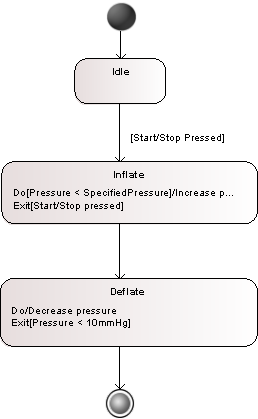
\includegraphics[width=0.5\textwidth]{pdfs/STM_Okklusion-crop.pdf}
\end{center}

\subsubsection{Setup}
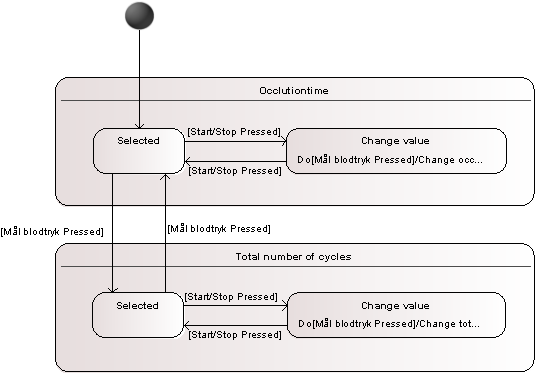
\includegraphics[width=\textwidth]{pdfs/STM_Setup-crop.pdf}
